\documentclass[manuscript, 12pt]{copernicus}

\usepackage{amsmath}
\usepackage{graphicx}
\usepackage{booktabs}
\usepackage{siunitx}
\usepackage{natbib}
\usepackage{hyperref}

\title{Design regret in clustered wind farms: how wind rose directionality and optimization thoroughness shape the cost of ignoring neighbors}

\Author[1]{Julian}{Quick}
\Author[1]{Pierre-Elouan}{R\'ethor\'e}

\affil[1]{Technical University of Denmark, Department of Wind and Energy Systems, Roskilde, Denmark}

\correspondence{Julian Quick (juqu@dtu.dk)}

\runningtitle{Design regret in clustered wind farms}
\runningauthor{Quick and R\'ethor\'e}

\begin{document}

\maketitle

\begin{abstract}
When a wind farm developer designs a layout in isolation, ignoring the wakes of potential neighboring farms, how much energy is sacrificed?
We define this loss as design regret and compute it using a bilevel optimization framework in which greedy adversarial neighbor placement maximizes regret against a re-optimized target layout.
Sweeping the two-parameter elliptical wind rose space of \citet{Hart2025}, with converged multistart optimization at $K = 500$ random restarts, we find that design regret varies six-fold: from 17\,GWh/yr (0.4\% of AEP) under moderate bidirectional conditions to 101\,GWh/yr (2.5\%) under concentrated unidirectional conditions.
Wind rose directionality---specifically the folding parameter controlling unidirectionality---is the primary driver.
Critically, we find that the computational effort required to accurately estimate design regret far exceeds standard practice: five random starts capture only 55--86\% of the converged regret, with bootstrap confidence intervals spanning $\pm$20\,GWh at $K = 5$.
We recommend a minimum of 300 multistart optimizations per strategy for reliable regret estimation.
Buffer distance analysis at converged optimization shows that regret decays with neighbor separation, but the decay rate itself depends on wind rose directionality: concentrated unidirectional sites require larger buffers than bidirectional ones.
\end{abstract}

\introduction

Offshore wind farms are designed in isolation, but operate in clusters.
This mismatch costs energy: wakes from neighboring farms---increasingly called ``wind theft'' \citep{Finseraas2024, Du2026}---persist for tens of kilometers \citep{Platis2018, Schneemann2020, Canadillas2022}, yet each farm's layout is typically optimized without knowledge of what will be built nearby.
The scale of the problem is substantial: inter-farm wake losses reduce offshore wind production by 13--15\% on the US east coast \citep{Rosencrans2024}, and cluster wake losses are projected to exceed the impact of a century of climate change in the North Sea \citep{Warder2025}.

In emerging offshore clusters, farms are designed and permitted sequentially, often by different developers \citep{Fliegner2025}.
A farm designed today must commit to a layout without knowing whether, when, or where neighbors will appear.
The standard approach is to optimize the layout in isolation---the ``liberal'' strategy.
If neighbors subsequently develop in positions that create significant wake interference, the liberal layout may be far from optimal for the realized conditions.

We formalize this loss as \emph{design regret}: the AEP difference between a layout designed with perfect neighbor foresight (conservative) and one designed in isolation (liberal), both evaluated under the same neighbor configuration:
\begin{equation}\label{eq:regret}
    R = \text{AEP}(\mathbf{x}^*_\text{cons}, \mathbf{n}) - \text{AEP}(\mathbf{x}^*_\text{lib}, \mathbf{n}).
\end{equation}
Regret isolates the cost of the design decision itself, separate from the total AEP reduction caused by neighbor wakes.

\citet{Quick2026omae} applied this framework to the Danish Energy Island cluster and found negligible design regret for all nine neighbor configurations.
This raised a question: is design regret generally negligible, or was this a property of that specific site?
We address this by systematically varying wind rose shape using the elliptical parameterization of \citet{Hart2025}, which separates directional concentration (parameter~$a$) from bidirectionality (parameter~$f$).

However, accurately computing regret reveals a computational challenge that has not been discussed in the wind farm optimization literature.
Layout optimization is highly multimodal \citep{Thomas2023, ValottaRodrigues2024}, and regret---as the \emph{difference} between two optimization outcomes---amplifies the effect of local optima.
We show that five random starts, more than many published studies employ, capture only 55--86\% of the converged regret, with confidence intervals comparable to the signal itself.
This convergence problem applies broadly to any study computing AEP differences between optimization strategies.

This paper makes three contributions:
\begin{enumerate}
    \item A convergence study demonstrating that 300+ multistart optimizations are needed for reliable regret estimation---an order of magnitude more than typical practice.
    \item A systematic sweep of the wind rose shape space showing that design regret varies six-fold with directionality, with concentrated unidirectional sites most vulnerable.
    \item Buffer distance analysis quantifying how neighbor separation reduces regret, and how the decay rate depends on wind rose shape.
\end{enumerate}

\section{Methods}\label{sec:methods}

\subsection{Problem formulation}

We consider a target wind farm of $N_t = 50$ IEA 15\,MW turbines ($D = 240$\,m, hub height 150\,m) within a fixed polygonal boundary derived from the Danish Energy Island concession zone.
Minimum inter-turbine spacing is $4D$.

The liberal layout $\mathbf{x}^*_\text{lib}$ maximizes AEP assuming no external turbines.
The conservative layout $\mathbf{x}^*_\text{cons}$ maximizes AEP accounting for specified neighbor positions~$\mathbf{n}$.
Both are evaluated with neighbors present to compute regret via Eq.~\eqref{eq:regret}.

By construction, $R \geq 0$ when both optimizations reach their global optima, since the liberal layout is a feasible (but generally suboptimal) conservative candidate.
We enforce this computationally through \emph{regret pooling}: the conservative AEP is computed as $\max(\text{best conservative AEP},\ \text{liberal AEP with neighbors})$, guaranteeing non-negative regret even with imperfect optimization.

\subsection{Wake model}

We use the \citet{Bastankhah2014} Gaussian deficit model with $k = 0.04$ and root-sum-of-squares superposition.
The simulation is implemented in JAX, enabling automatic differentiation through the wake model for gradient-based layout optimization.

\subsection{Wind rose parameterization}

Wind rose shape is parameterized using the elliptical model of \citet{Hart2025}:
\begin{itemize}
    \item Shape parameter $a$: controls concentration ($a = 1/\sqrt{\pi} \approx 0.564$ gives uniform).
    \item Folding parameter $f \in [0,1]$: controls symmetry ($f = 0$ bidirectional, $f = 1$ unidirectional).
\end{itemize}
The prevailing direction is fixed at 270\textdegree{} and wind speed at 9\,m/s across 24 sectors.
We sweep $a \in \{0.3, 0.4, 0.5, 0.6, 0.7, 0.8, 0.9\}$ and $f \in \{0.0, 0.25, 0.5, 0.75, 1.0\}$ (35 combinations).

Fitting the DEI wind rose with the elliptical model yields $a \approx 0.64$, $f \approx 0.38$ ($R^2 = 0.84$), placing it in the moderate-concentration, partially-bidirectional regime.

\subsection{Adversarial neighbor placement}

Neighbors are placed using a greedy grid search.
A candidate grid with 5$D$ spacing extends 50$D$ from the target boundary.
At each of 30 steps, the candidate maximizing incremental regret is selected.
Each candidate evaluation requires a full $K$-start conservative optimization.

This greedy approach provides an \emph{upper bound} on design regret---it does not represent realistic neighbor behavior, but identifies the most vulnerable directions and the maximum cost of designing in isolation.

\subsection{Multistart optimization and convergence}

Each layout optimization uses gradient-based SGD with 5000 iterations.
Following the convergence analysis of \citet{Quick2026omae}, who found that $\sim$400 starts are needed for liberal layout convergence with 66 turbines, we perform a dedicated convergence study (Section~\ref{sec:convergence}) for the regret computation.

Based on this study, production runs use $K = 500$ random starts for the conservative optimization and $K_\text{lib} = 100$ for the liberal optimization, with regret pooling to guarantee $R \geq 0$.

\section{Results}\label{sec:results}

\subsection{Convergence study: how many starts are enough?}\label{sec:convergence}

We sweep the number of conservative starts $K$ from 1 to 2000 for three configurations spanning the wind rose space (Fig.~\ref{fig:convergence}).
A 5$\times$5 reference neighbor farm (25 turbines at 7$D$ spacing) is placed at a fixed bearing and distance for each configuration.

\begin{figure}[t]
    \centering
    
\includegraphics[width=\textwidth]{figures/convergence.png}
    \caption{Convergence of design regret with number of multistart optimizations~$K$.
    Dashed gray: converged value ($K = 2000$).
    Dotted blue: $K = 5$ value.
    All three configurations stabilize by $K \approx 300$.}
    \label{fig:convergence}
\end{figure}

At $K = 5$, regret captures only 55--86\% of the converged value depending on configuration (Table~\ref{tab:convergence}).
The moderate bidirectional case is the worst: $K = 5$ finds only 55\% of the true regret because the optimization landscape contains many local optima with similar isolated-AEP but very different neighbor-present AEP.
All three configurations stabilize by $K = 300$, with no change from $K = 300$ to $K = 2000$.

\begin{table}[t]
    \centering
    \caption{Design regret (GWh/yr) at selected $K$ values for three test configurations.}
    \label{tab:convergence}
    \begin{tabular}{lccccc}
        \toprule
        Configuration & $K = 5$ & $K = 100$ & $K = 300$ & $K = 500$ & $K = 2000$ \\
        \midrule
        Conc.\ unidir, 5$D$ & 15.9 & 15.9 & 26.2 & 26.2 & 26.6 \\
        Conc.\ unidir, 20$D$ & 67.9 & 67.9 & 79.3 & 79.3 & 79.3 \\
        Mod.\ bidir, 5$D$ & 24.1 & 43.1 & 43.6 & 43.6 & 43.6 \\
        \bottomrule
    \end{tabular}
\end{table}

SGD iteration convergence is much faster: at $K = 500$, regret is within 3\% of the 10000-iteration value at 5000 iterations.
We use $K = 500$ and 5000 iterations for all subsequent analyses.

\subsection{Wind rose shape controls design regret}

Figure~\ref{fig:heatmap} shows design regret across the full $(a, f)$ parameter space at $K = 500$.
Regret ranges from 17.2\,GWh (0.4\% of AEP) at $a = 0.5$, $f = 0.0$ to 100.6\,GWh (2.5\%) at $a = 0.9$, $f = 1.0$---a six-fold range.

\begin{figure}[t]
    \centering
    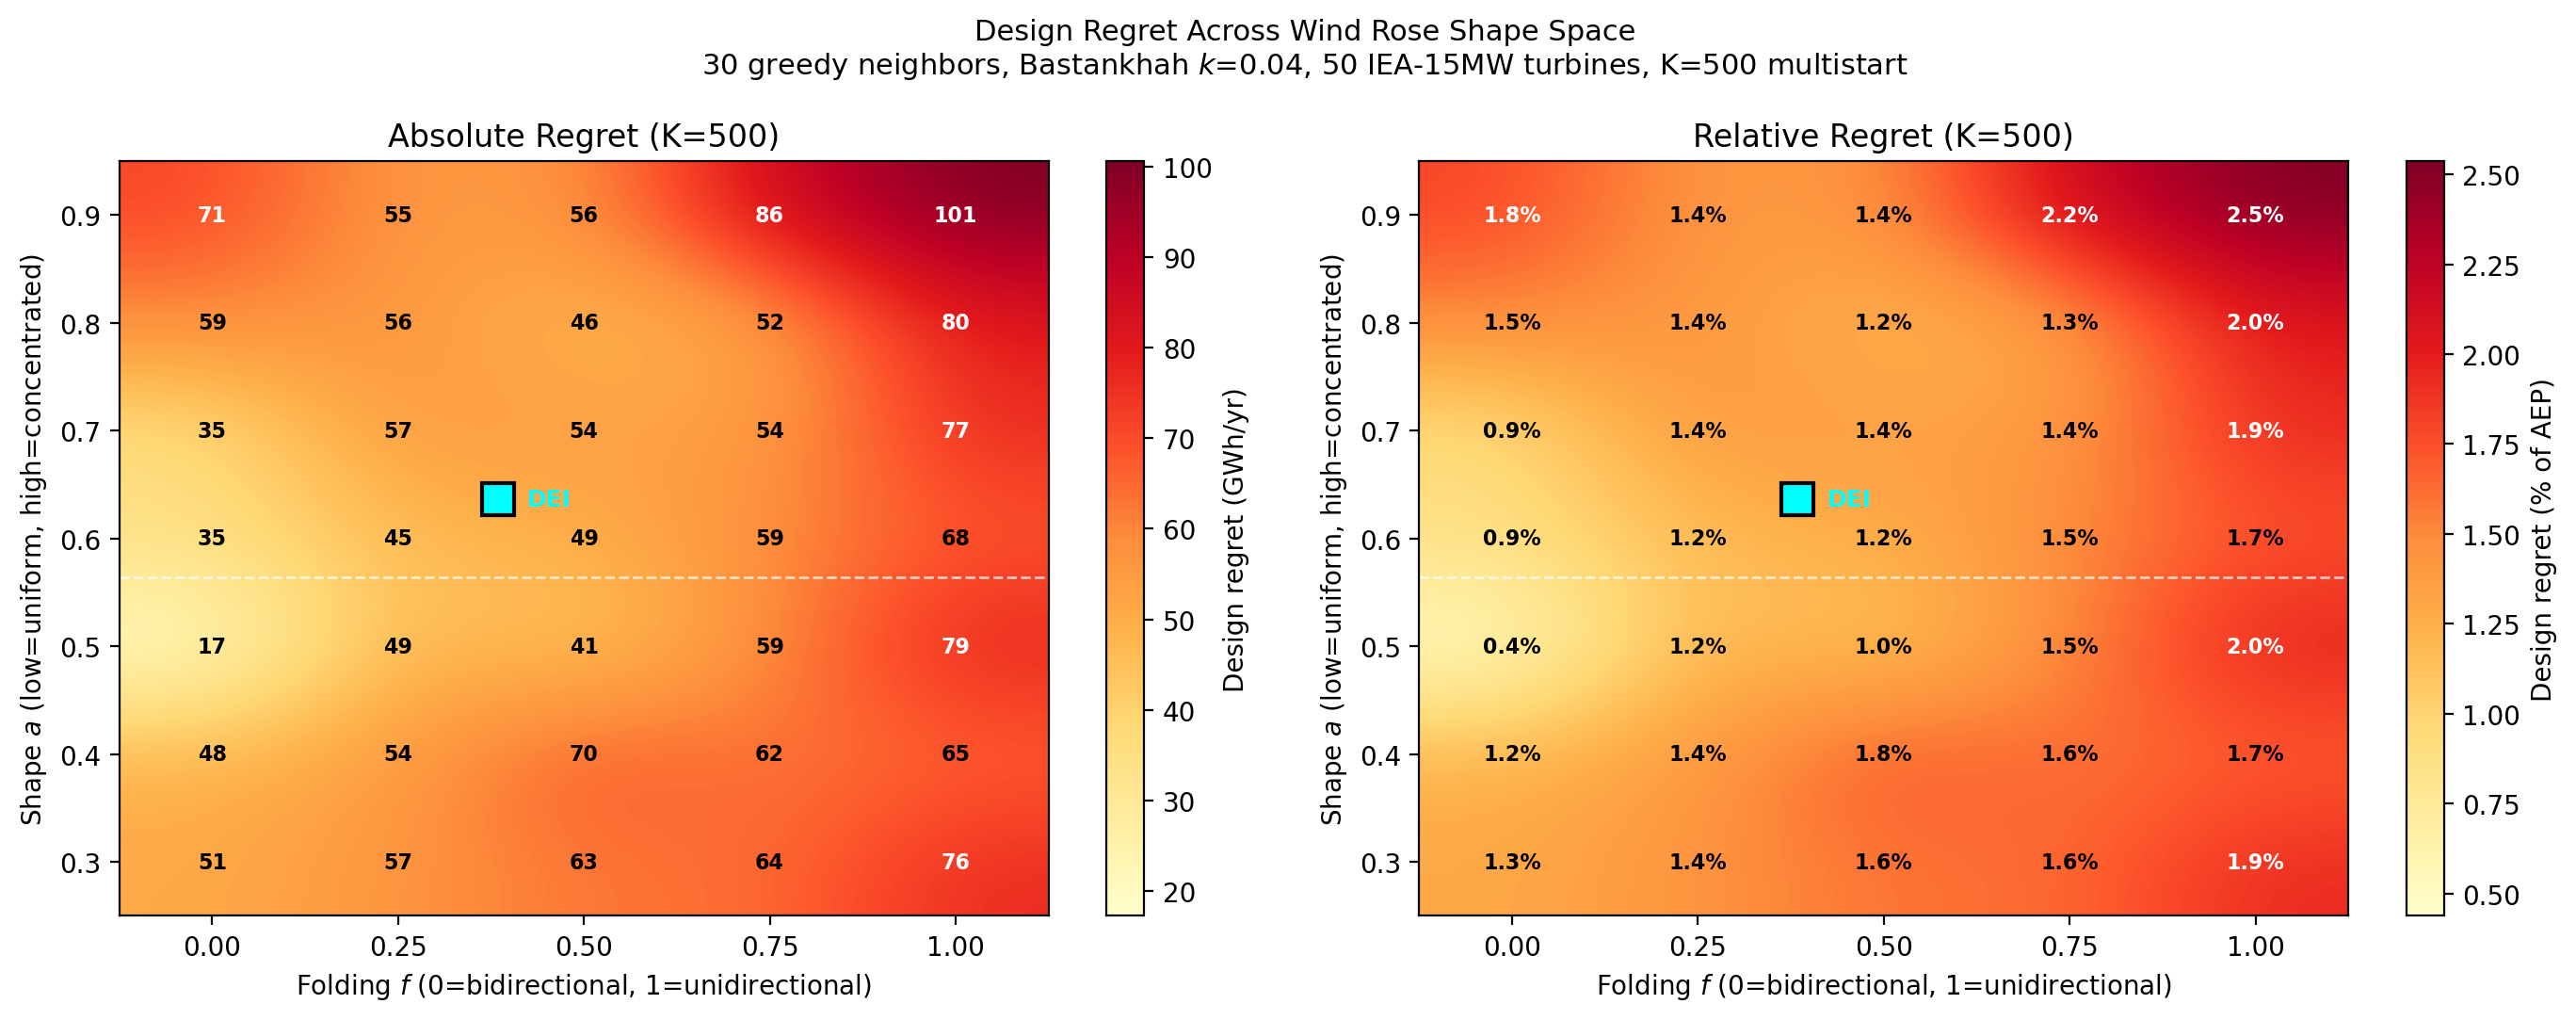
\includegraphics[width=\textwidth]{figures/edrose_heatmap_k500.png}
    \caption{Design regret across the elliptical wind rose shape space at $K = 500$.
    Left: absolute (GWh/yr). Right: relative (\% of AEP).
    The cyan square marks the fitted DEI wind rose ($a \approx 0.64$, $f \approx 0.38$).}
    \label{fig:heatmap}
\end{figure}

The folding parameter $f$ is the dominant factor.
Mean regret increases monotonically with $f$: from 45.2\,GWh at $f = 0.0$ (bidirectional) to 77.9\,GWh at $f = 1.0$ (unidirectional), as shown in Fig.~\ref{fig:regret_vs_f}.
Concentration ($a$) has a weaker, non-monotonic effect.

\begin{figure}[t]
    \centering
    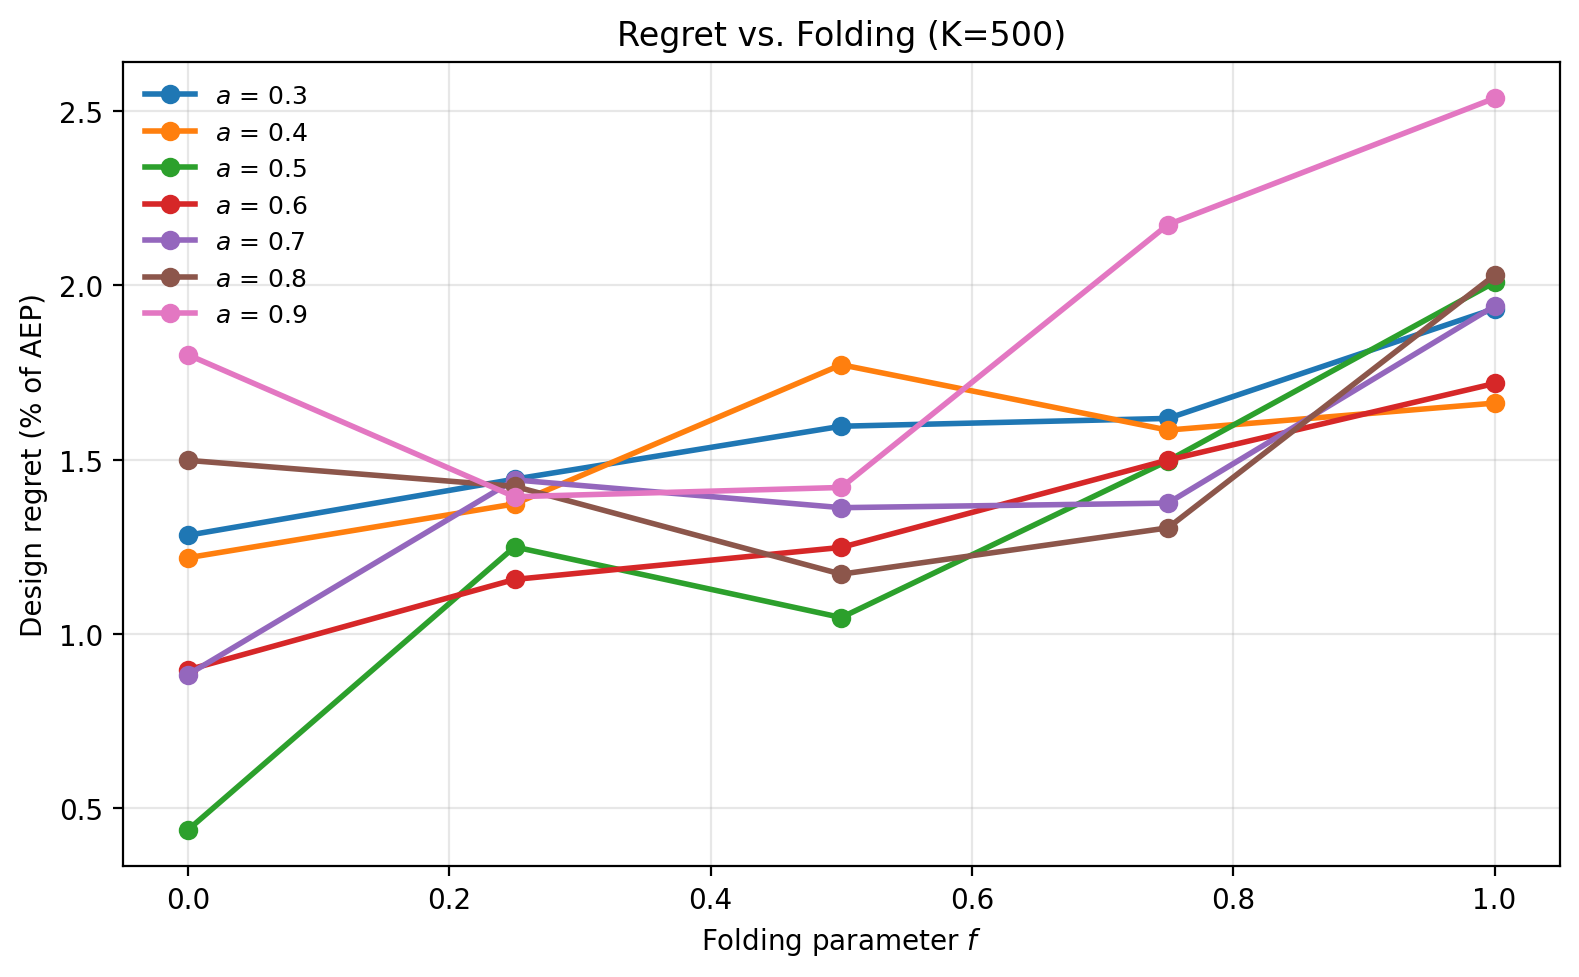
\includegraphics[width=0.65\textwidth]{figures/regret_vs_f.png}
    \caption{Regret vs.\ folding parameter $f$ at each concentration level $a$ ($K = 500$).
    The monotonic increase with $f$ is consistent across all~$a$.}
    \label{fig:regret_vs_f}
\end{figure}

The physical mechanism is straightforward.
Unidirectional wind creates a single wake corridor from each neighbor.
The liberal layout, optimized without knowledge of this corridor, cannot avoid it.
The conservative layout can shift turbines laterally.
Under bidirectional conditions, wakes arrive from opposing directions and no lateral shift helps---regret is inherently limited.

The DEI wind rose ($a \approx 0.64$, $f \approx 0.38$) falls in the moderate-regret region of the shape space, consistent with the negligible design tradeoffs found by \citet{Quick2026omae}.

\subsection{Buffer distance modulates regret}

Figure~\ref{fig:buffer} shows how regret decays with buffer distance at $K = 500$ for three representative wind roses.

\begin{figure}[t]
    \centering
    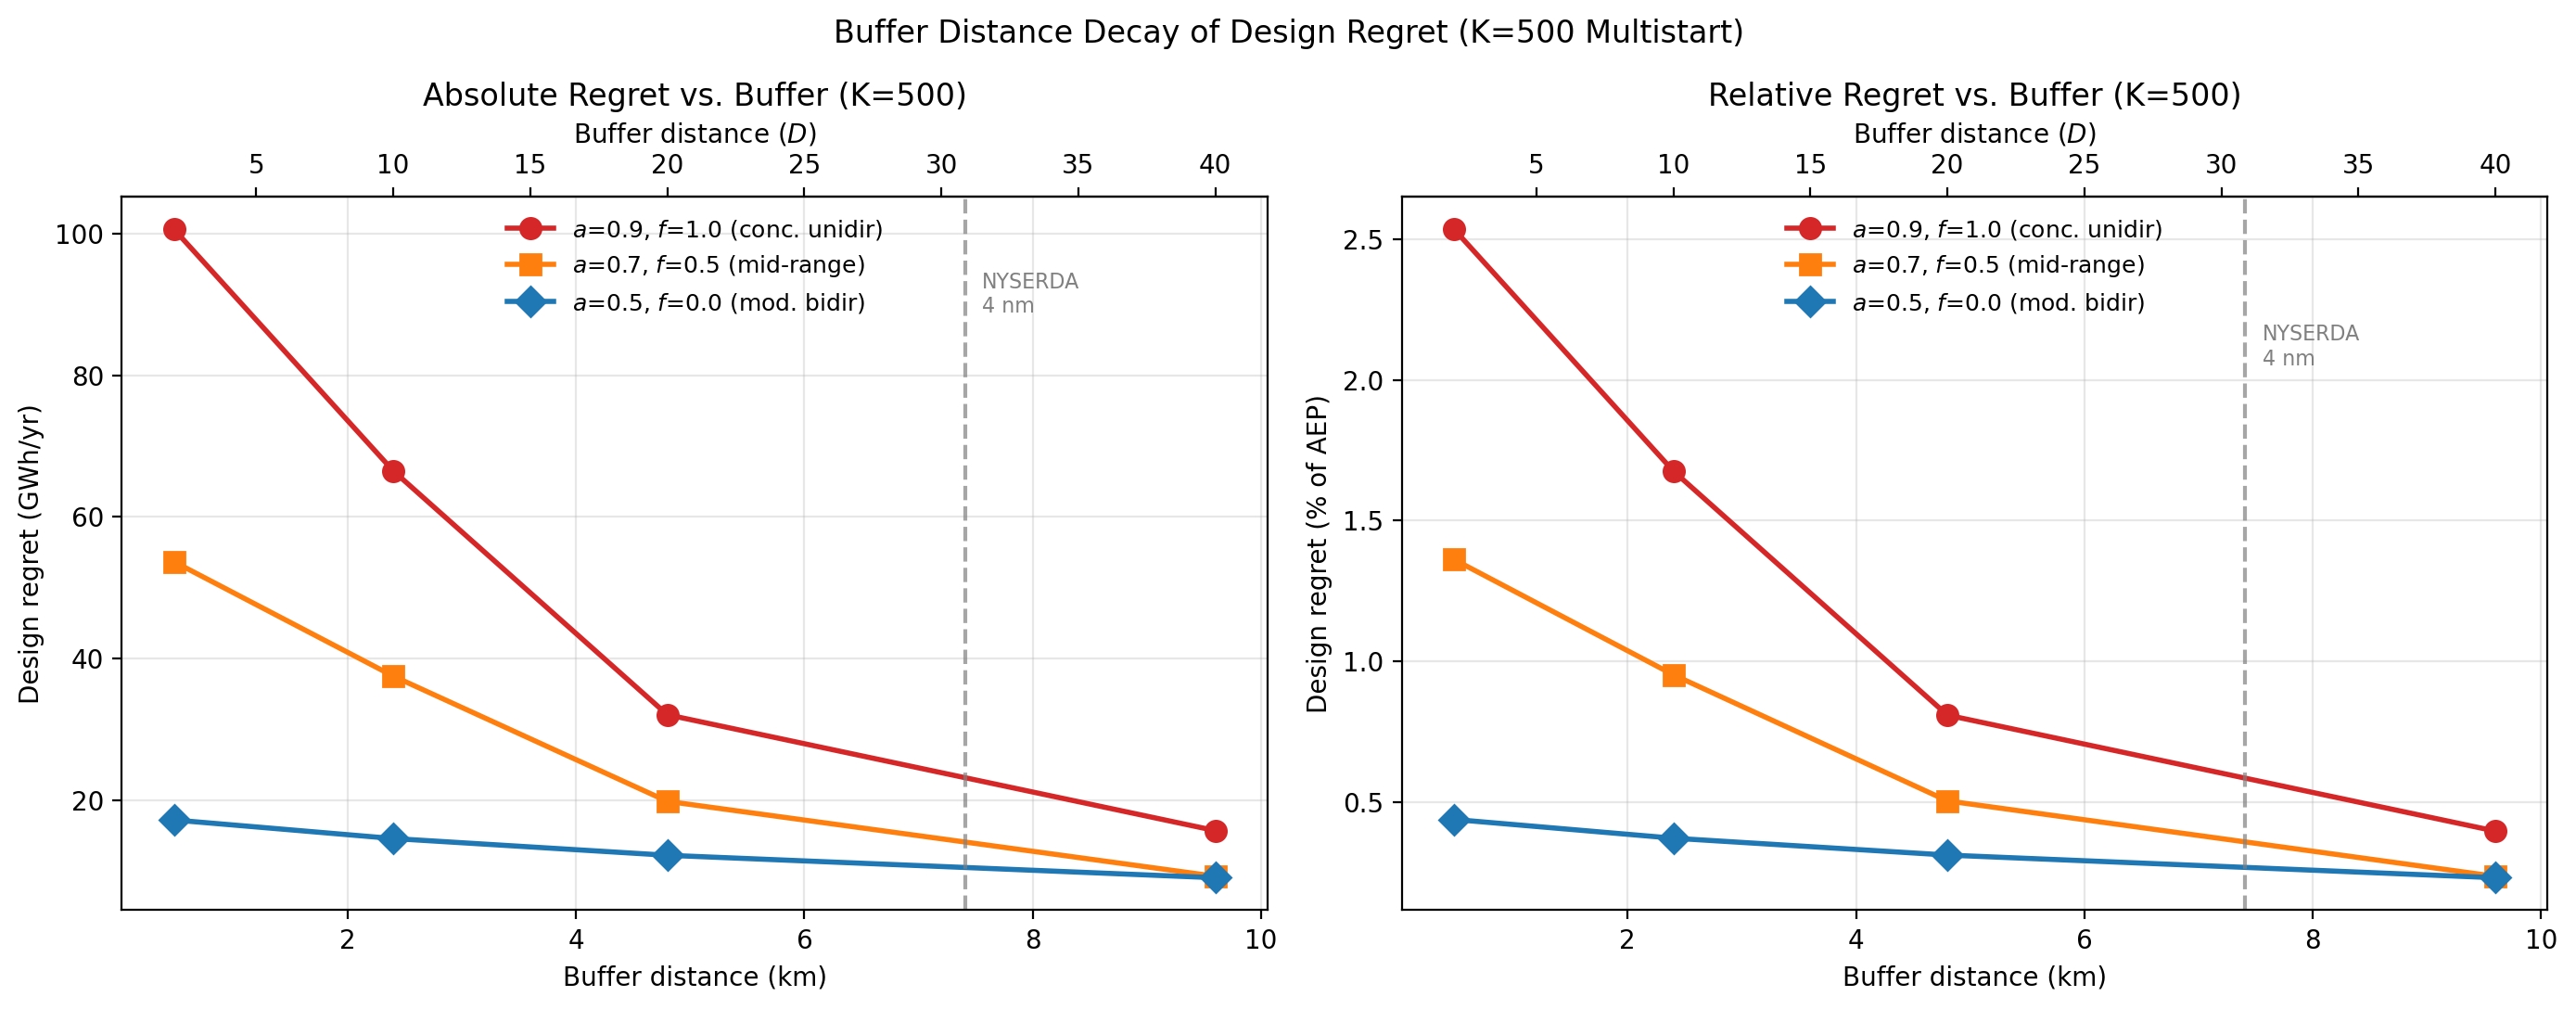
\includegraphics[width=\textwidth]{figures/buffer_decay_k500.png}
    \caption{Regret vs.\ buffer distance at $K = 500$.
    Decay rate depends on wind rose directionality.
    The NYSERDA-recommended 4\,nm inter-farm spacing is marked.}
    \label{fig:buffer}
\end{figure}

For the concentrated unidirectional case ($a = 0.9$, $f = 1.0$), regret declines from 100.6\,GWh at 2$D$ to 15.7\,GWh at 40$D$ (9.6\,km)---a steep but incomplete decay, with 16\% residual regret.
The bidirectional case ($a = 0.5$, $f = 0.0$) decays more gently, from 17.2 to 9.1\,GWh, because regret is already low.

These results imply that a single buffer distance standard is inefficient: concentrated unidirectional sites may need 30--40$D$ buffers ($\sim$7--10\,km), while bidirectional sites need minimal separation.

\subsection{Effect of optimization depth on greedy grid results}

Figure~\ref{fig:k5_vs_k500} compares the 35-case edrose sweep at $K = 5$ and $K = 500$.
Unlike the convergence study on a single fixed neighbor, the greedy grid search produces noisier but less systematically biased results: individual K=5 ratios range from 71\% to 138\% of K=500 values, with a mean ratio of 103\%.

\begin{figure}[t]
    \centering
    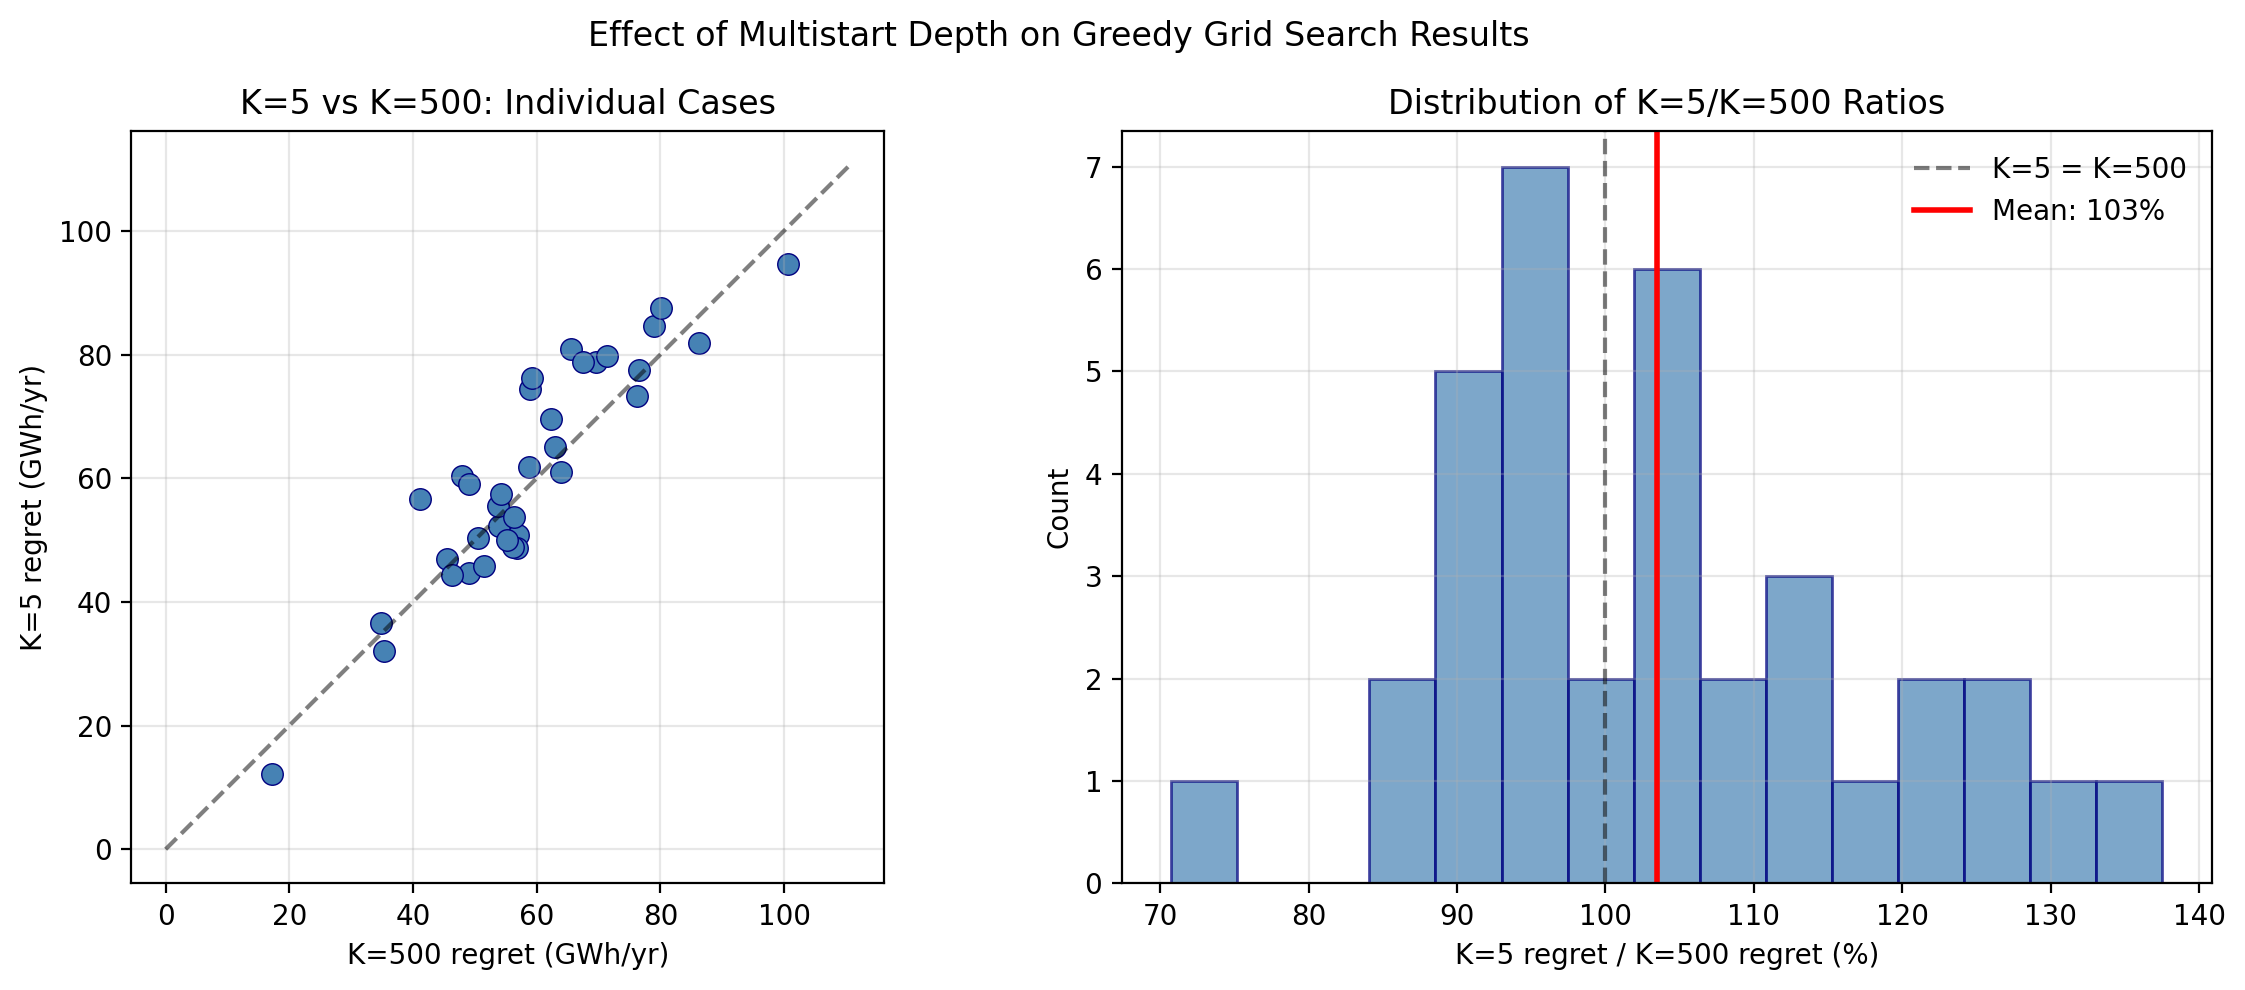
\includegraphics[width=\textwidth]{figures/k5_vs_k500.png}
    \caption{Comparison of $K = 5$ vs.\ $K = 500$ greedy grid regret across 35 wind rose configurations.
    Left: scatter plot. Right: histogram of $K = 5$/$K = 500$ ratios.
    The greedy search absorbs some K-insufficiency by finding different (sometimes better) greedy paths.}
    \label{fig:k5_vs_k500}
\end{figure}

This occurs because the greedy grid search is path-dependent: at each step, different $K$ values may select different ``best'' candidates, leading to different subsequent neighbor configurations.
The greedy algorithm thus partially compensates for K-insufficiency at any single step, unlike a fixed-neighbor evaluation where under-optimization always underestimates regret.
Nevertheless, the $K = 500$ results should be preferred for quantitative claims.

\subsection{Directional vulnerability (preliminary, $K = 5$)}\label{sec:cross-section-preliminary}

Preliminary regret cross-sections at $K = 5$ (placing a 5$\times$5 reference farm at 24 bearings $\times$ 7 distances) suggest an ``ambush effect'': peak vulnerability occurs at oblique angles to the dominant wind direction, not along it.
For example, under concentrated unidirectional conditions ($a = 0.9$, $f = 1.0$, dominant direction 270\textdegree), the highest regret appears near 105\textdegree---nearly perpendicular.

This pattern is physically plausible: the liberal layout is pre-adapted to the dominant direction and therefore partially resilient to aligned neighbors.
Off-axis neighbors exploit the layout's ``blind spots.''
However, these results are at $K = 5$, which the convergence study shows captures only 55--86\% of converged regret.
Cross-sections at converged $K$ are in computation and will be reported in a future revision.

\section{Discussion}\label{sec:discussion}

\subsection{The convergence problem is real and underappreciated}

Our most practically important finding may be methodological.
Accurately computing design regret requires far more optimization effort than previously recognized.
At $K = 5$, regret estimates can be off by a factor of two.

The root cause is the interaction between multimodality and differencing.
Each individual optimization may find a ``good'' local optimum within a few percent of the global best.
But the \emph{difference} between two such solutions amplifies relative errors---a form of catastrophic cancellation that is well-known in numerical analysis but has not been discussed in the wind farm optimization literature.

This problem applies to any study computing AEP differences between strategies: robust optimization, Pareto analysis, or value-of-information calculations.
We recommend that such studies report convergence behavior with respect to the number of random starts, and use $K \geq 300$ for reliable results with farm sizes of $\sim$50 turbines.

\subsection{Physical drivers of design regret}

The six-fold range in regret across the wind rose space has a clear physical interpretation.
Design regret requires two conditions: (1)~neighbor wakes must affect the target farm, and (2)~a redesigned layout must substantially reduce the impact.

Unidirectional concentrated wind maximizes condition~(2): neighbor wakes arrive from a narrow angular range, so the conservative optimizer can shift turbines laterally out of the wake corridor.
Under bidirectional conditions, wakes arrive from opposing directions and no single rearrangement can escape them all, limiting the benefit of neighbor knowledge.

\subsection{Implications for cluster planning}

Sites with concentrated unidirectional wind (high $a$, high $f$) face the highest design regret and benefit most from early coordination between developers.
Buffer distance standards should account for wind rose directionality: a fixed 4\,nm buffer may be adequate for bidirectional sites but insufficient for strongly directional ones.

The computational burden of converged regret estimation is substantial but tractable with GPU-accelerated differentiable wake simulations.
For a 50-turbine farm at $K = 500$, each wind rose configuration requires $\sim$10\,000 gradient-based layout optimizations (500 conservative + 100 liberal + screening), taking approximately 2~hours on a single MI250X GCD.

\subsection{Limitations}

\paragraph{Wake model.} We use the Bastankhah Gaussian model with root-sum-of-squares superposition.
More sophisticated models with turbulence-dependent expansion (e.g., TurbOPark) may change absolute magnitudes.
Preliminary $K = 5$ comparisons suggest TurbOPark produces 4--10$\times$ higher regret, but this has not been verified at converged~$K$.

\paragraph{Adversarial assumption.} The greedy grid search places individual turbines to maximize regret---an adversarial upper bound, not a realistic scenario.
A self-interested neighbor optimizing its own AEP may produce different regret patterns.
Preliminary $K = 5$ results suggest self-interested neighbors can actually produce \emph{higher} regret than fixed reference farms at the same location, because AEP-optimal neighbor placement concentrates turbines in high-wind positions upwind of the target.
This finding warrants further investigation at converged~$K$.

\paragraph{Constant wind speed.} All analyses use 9\,m/s across all directions.
Real sites have speed--direction correlations that could amplify regret through the cubic power relationship.

\paragraph{Single farm geometry.} Results may depend on the specific DEI-derived polygonal boundary.

\paragraph{Cross-section convergence.} The directional vulnerability analysis (Section~\ref{sec:cross-section-preliminary}) is at $K = 5$.
While the qualitative ``ambush effect'' is physically plausible, the magnitudes should be treated as preliminary.

\conclusions

\begin{enumerate}
    \item \textbf{Standard multistart practice drastically underestimates design regret.}
    Five random starts capture only 55--86\% of the converged regret for a 50-turbine farm.
    Bootstrap confidence intervals at $K = 5$ exceed $\pm$20\,GWh---comparable to the signal itself.
    We identify $K = 300$ as the minimum for reliable estimation.

    \item \textbf{Design regret varies six-fold across the wind rose shape space.}
    At converged optimization ($K = 500$), adversarial neighbor placement produces regret from 17\,GWh/yr (0.4\% of AEP) under moderate bidirectional conditions to 101\,GWh/yr (2.5\%) under concentrated unidirectional conditions.
    Wind rose directionality (the folding parameter~$f$) is the primary driver.

    \item \textbf{Buffer distance requirements are wind-rose-dependent.}
    Regret from concentrated unidirectional sites decays steeply with buffer distance but retains 16\% residual at 40$D$ (9.6\,km).
    Bidirectional sites show little sensitivity to buffer.
    One-size-fits-all buffer zones are inefficient.

    \item \textbf{Preliminary evidence suggests directional vulnerability peaks at oblique angles} to the dominant wind (the ``ambush effect''), consistent with the liberal layout being pre-adapted to the dominant direction.
    This warrants further investigation at converged optimization depth.
\end{enumerate}

The Danish Energy Island, with its moderately bidirectional wind rose ($f \approx 0.38$), sits in the low-regret region---consistent with the negligible design tradeoffs found by \citet{Quick2026omae}.
Sites with strongly unidirectional wind are substantially more vulnerable to uncoordinated cluster development.

\codedataavailability{
The simulation framework (pixwake) and all analysis scripts are available at \url{https://github.com/kilojoules/cluster-tradeoffs}.
The elliptical wind rose parameterization uses the edrose package \citep{Hart2025}, available at \url{https://github.com/kilojoules/edrose}.
}

\authorcontribution{
JQ designed the study, developed the simulation framework, performed all computations, and wrote the manuscript.
PER supervised the research and contributed to methodology and manuscript revision.
}

\competinginterests{
The authors declare no competing interests.
}

\begin{acknowledgements}
Computational resources were provided by the LUMI supercomputer, hosted by CSC (Finland) and the LUMI consortium.
\end{acknowledgements}

\bibliographystyle{copernicus}
\bibliography{references}

\end{document}
